\documentclass[a4paper, final]{article}

% ============================================================
% settings
% ============================================================
\usepackage[russian]{babel}
\usepackage{fontspec}
\setmainfont{Times New Roman}
\newfontfamily\cyrillicfonttt{Courier New}
\usepackage[14pt]{extsizes}
\usepackage[left=20mm, top=20mm, right=20mm, bottom=20mm, footskip=10mm]{geometry}
\usepackage{ragged2e}
\usepackage{indentfirst}
\usepackage{graphicx}
\usepackage{caption}
\usepackage{xcolor}
\usepackage{listings}
\usepackage{booktabs}
\usepackage{hyperref}
\usepackage{amsmath}
\usepackage{amssymb}
\usepackage{array}

\definecolor{link_color}{HTML}{0000EE}

\hypersetup{
    colorlinks=true,
    linkcolor=link_color,
    urlcolor=link_color,
    citecolor=link_color
}

\lstset{
    language=Python,
    basicstyle=\cyrillicfonttt\small,
    numbers=left,
    numberstyle=\tiny\color{gray},
    keywordstyle=\color{blue}\bfseries,
    commentstyle=\color{gray}\itshape,
    stringstyle=\color{red},
    frame=single,
    captionpos=b,
    breaklines=true,
    breakatwhitespace=false,
    showstringspaces=false,
    keepspaces=true,
    columns=flexible,
    fontadjust=true,
    basewidth={0.5em,0.45em},
    tabsize=4,
}

\begin{document}

% ============================================================
% title page
% ============================================================
{
\thispagestyle{empty}
\begin{center}
    \hfill \break
    \hfill \break
    МИНИСТЕРСТВО НАУКИ И ВЫСШЕГО ОБРАЗОВАНИЯ РОССИЙСКОЙ ФЕДЕРАЦИИ\\[5 pt]
    Федеральное государственное автономное образовательное учреждение высшего образования
    «Санкт-Петербургский политехнический университет Петра Великого»\\[10 pt]
    Институт компьютерных наук и кибербезопасности\\[5 pt]
    Направление: 02.03.01 Математика и компьютерные науки\\[30pt]

    {\large Отчет по дисциплине: «Вычислительная математика»}\\[30 pt]
    \LARGE\bf «Лабораторная работа №4».
\end{center}

\vspace{110 pt}

\begin{tabular*}{460pt}{@{\extracolsep{\fill}} l r}
     Студент,\tabularnewline группы 5130201/40003 \hspace{50pt}&  \line(1,0){100} \quad Адиатуллин Т. Р.\\
     & \\
     Руководитель,\tabularnewline Преподаватель & \line(1,0){121.5} \quad Пак В. Г.\\
     & \\
     & \\
     & \\
     & \guillemotleft \line(1,0){30} \guillemotright \line(1,0){100} \, 2026 \,г.
\end{tabular*} \\

\vfill

\begin{center}
    Санкт-Петербург, 2026
\end{center}
\newpage
}

\tableofcontents
\newpage

% ============================================================
% section 1
% ============================================================
\section{Постановка задачи}

\textbf{Тема:} численное интегрирование.

\textbf{Цель:} научиться приближённо оценивать значения определённых интегралов по
квадратурным формулам Ньютона-Котеса и Гаусса.

\textbf{Задание:}
\begin{enumerate}
    \item Вычислить приближённо интеграл по формуле Ньютона-Котеса с данным значением~$n$,
          оценить погрешность приближения с помощью остаточного члена.
    \item Вычислить приближённо интеграл по формуле Гаусса с данным значением~$n$,
          оценить погрешность приближения по более точному значению интеграла,
          вычисленному по формуле Ньютона-Лейбница (при возможности интегрирования).
\end{enumerate}

Требуется вычислить интеграл:
\[
I = \int_{1}^{2{,}5} \ln\!\left(x^2 + \sqrt{x^4 + 1}\right)dx.
\]
Данные варианта: $n = 5$ (для формулы Ньютона-Котеса), $n = 4$ (для формулы Гаусса).

\newpage

% ============================================================
% section 2 — theory
% ============================================================
\section{Теоретические сведения}

\subsection{Квадратурные формулы Ньютона-Котеса}

Квадратурные формулы Ньютона-Котеса относятся к формулам интерполяционного типа.
Подынтегральную функцию аппроксимируют на промежутке интегрирования $[a,b]$
некоторой функцией, интеграл от которой легко вычисляется. Тогда приближённое
значение искомого интеграла равно интегралу от интерполирующей функции.

Оценку интеграла по формуле Ньютона-Котеса можно записать в виде:
\begin{equation}\label{eq:nk}
\int_a^b f(x)\,dx \approx \sum_{i=0}^{n-1} C_i^{(n)}\, f(x_i) + R^{(n)}(\xi),
\end{equation}
где $x_i$ --- узлы квадратуры, они же узлы интерполяции $x_i = a + ih$,
$h = \dfrac{b-a}{n-1}$. Коэффициенты $C_i^{(n)}$ и остаточные члены $R^{(n)}(\xi)$
для разных $n$ приведены в таблице~\ref{tab:nk}.

\begin{table}[h!]
\centering
\caption{Коэффициенты $C_i^{(n)}$ и остаточные члены формул Ньютона-Котеса.}
\label{tab:nk}
\renewcommand{\arraystretch}{1.4}
\begin{tabular}{|c|c|c|c|c|c|c|}
\hline
$n$ & $C_0^{(n)}$ & $C_1^{(n)}$ & $C_2^{(n)}$ & $C_3^{(n)}$ & $C_4^{(n)}$
    & $R^{(n)}(\xi)$ \\
\hline
2 & $\dfrac{1}{2}$ & $\dfrac{1}{2}$ & --- & --- & ---
  & $-\dfrac{b-a}{12}h^2 f''(\xi)$ \\[6pt]
\hline
3 & $\dfrac{1}{6}$ & $\dfrac{4}{6}$ & $\dfrac{1}{6}$ & --- & ---
  & $-\dfrac{b-a}{90}h^4 f^{(4)}(\xi)$ \\[6pt]
\hline
4 & $\dfrac{1}{8}$ & $\dfrac{3}{8}$ & $\dfrac{3}{8}$ & $\dfrac{1}{8}$ & ---
  & $-\dfrac{3(b-a)}{80}h^4 f^{(4)}(\xi)$ \\[6pt]
\hline
5 & $\dfrac{14}{90}$ & $\dfrac{64}{90}$ & $\dfrac{24}{90}$ & $\dfrac{64}{90}$
  & $\dfrac{14}{90}$
  & $-\dfrac{8(b-a)}{945}h^6 f^{(6)}(\xi)$ \\[6pt]
\hline
\end{tabular}
\end{table}

По $R^{(n)}(\xi)$ можно оценивать предельную погрешность.

\subsection{Квадратурные формулы Гаусса}

Пусть надо вычислить приближённо интеграл
\begin{equation}\label{eq:gauss_int}
I = \int_a^b f(x)\,\rho(x)\,dx,
\end{equation}
где $\rho(x)$ --- весовая функция. Квадратура Гаусса --- это формула приближённого
вычисления интеграла~\eqref{eq:gauss_int}, узлы которой~$t_i$ являются корнями
многочлена $\omega_n(t)$, ортогонального на $[a,b]$ с весом $\rho(x)$.

В таблице~\ref{tab:gauss} приведены узлы $t_i$ и веса $A_i$ квадратур Гаусса для
интеграла $\displaystyle\int_{-1}^{1} f(t)\,dt$ (т.е.\ $\rho(t) \equiv 1$).

\begin{table}[h!]
\centering
\caption{Узлы $t_i$ и веса $A_i$ квадратур Гаусса (на $[-1,1]$).}
\label{tab:gauss}
\renewcommand{\arraystretch}{1.3}
\begin{tabular}{|c|c|c|}
\hline
$n$ & $\pm\,t_i$ & $A_i$ \\
\hline
\multirow{2}{*}{4}
  & $t_{1,4} = 0{,}861136312$ & $A_{1,4} = 0{,}347854845$ \\
  & $t_{2,3} = 0{,}339981044$ & $A_{2,3} = 0{,}652145155$ \\
\hline
\end{tabular}
\end{table}

Если надо вычислить интеграл на отрезке $[a,b]$, то коэффициенты $A_i$ остаются
прежними, но узлы надо пересчитать по формуле:
\begin{equation}\label{eq:gauss_nodes}
x_i = \frac{a+b}{2} + \frac{b-a}{2}\,t_i.
\end{equation}
Тогда:
\begin{equation}\label{eq:gauss_formula}
\int_a^b f(x)\,dx \approx \frac{b-a}{2}\sum_{i=1}^{n} A_i\,f(x_i).
\end{equation}

\newpage

% ============================================================
% section 3 — Newton-Cotes
% ============================================================
\section{Формула Ньютона-Котеса ($n = 5$)}

\subsection{Шаг разбиения и узлы интерполяции}

Интеграл вычисляется на отрезке $[a,b] = [1;\;2{,}5]$ при $n = 5$ узлах.
Шаг разбиения:
\[
h = \frac{b - a}{n - 1} = \frac{2{,}5 - 1}{4} = 0{,}375.
\]

Узлы интерполяции $x_i = a + i\,h$, $i = 0, 1, 2, 3, 4$:
\[
x_0 = 1{,}000, \quad x_1 = 1{,}375, \quad x_2 = 1{,}750,
\quad x_3 = 2{,}125, \quad x_4 = 2{,}500.
\]

\subsection{Значения подынтегральной функции}

Обозначим $f_i = f(x_i)$. Значения функции
$f(x) = \ln\!\left(x^2 + \sqrt{x^4+1}\right)$ в узлах приведены в таблице~\ref{tab:nc_vals}.

\begin{table}[h!]
\centering
\caption{Узлы и значения функции для формулы Ньютона-Котеса ($n=5$).}
\label{tab:nc_vals}
\begin{tabular}{|c|c|c|}
\hline
$i$ & $x_i$ & $f_i = f(x_i)$ \\
\hline
0 & 1,0000 & 0,881374 \\
1 & 1,3750 & 1,393624 \\
2 & 1,7500 & 1,838028 \\
3 & 2,1250 & 2,212732 \\
4 & 2,5000 & 2,532068 \\
\hline
\end{tabular}
\end{table}

На листинге~\ref{lst:nc_setup} приведён код вычисления узлов и значений функции.

\begin{lstlisting}[caption={Узлы и значения функции}, label=lst:nc_setup]
import numpy as np

f = lambda x: np.log(x**2 + np.sqrt(x**4 + 1))
a, b = 1.0, 2.5
n = 5
h = (b - a) / (n - 1)  # h = 0.375

nodes = [a + i * h for i in range(n)]
print(f"h = {h}")
for i, xi in enumerate(nodes):
    print(f"x_{i} = {xi:.4f},  f(x_{i}) = {f(xi):.6f}")
\end{lstlisting}

\subsection{Вычисление интеграла}

При $n = 5$ из формулы~\eqref{eq:nk} и таблицы~\ref{tab:nk} получаем формулу Буля:
\[
I^* = \frac{b-a}{90}\bigl[14f_0 + 64f_1 + 24f_2 + 64f_3 + 14f_4\bigr]
    = \frac{2h}{45}\bigl[7f_0 + 32f_1 + 12f_2 + 32f_3 + 7f_4\bigr].
\]

Подставляем значения:
\begin{align*}
&7f_0 + 32f_1 + 12f_2 + 32f_3 + 7f_4 \\
&= 7 \cdot 0{,}881374 + 32 \cdot 1{,}393624 + 12 \cdot 1{,}838028
   + 32 \cdot 2{,}212732 + 7 \cdot 2{,}532068 \\
&= 6{,}169618 + 44{,}595968 + 22{,}056336 + 70{,}807424 + 17{,}724476
 = 161{,}353822.
\end{align*}

Итоговое значение:
\[
\boxed{I^*_\text{НК} = \frac{2 \cdot 0{,}375}{45} \cdot 161{,}353822 \approx 2{,}689230.}
\]

На листинге~\ref{lst:nc_calc} приведён соответствующий код.

\begin{lstlisting}[caption={Вычисление интеграла по формуле Буля ($n=5$)}, label=lst:nc_calc]
fvals = [f(xi) for xi in nodes]
# Koeffitsienty dlya n=5 (formula Bulya)
C = np.array([14, 64, 24, 64, 14])

total  = np.dot(C, fvals)
I_star = (b - a) / 90 * total

print(f"14f0+64f1+24f2+64f3+14f4 = {total:.6f}")
print(f"I* = (b-a)/90 * S = {I_star:.6f}")
\end{lstlisting}

\subsection{Оценка погрешности}

Остаточный член формулы Буля (из таблицы~\ref{tab:nk}):
\[
R^{(5)}(\xi) = -\frac{8(b-a)}{945}\,h^6\,f^{(6)}(\xi), \quad \xi \in [a,b].
\]

Отсюда оценка предельной погрешности:
\[
\bigl|R^{(5)}\bigr| \leq \frac{8(b-a)}{945}\,h^6\,M_6,
\qquad M_6 = \max_{x\in[a,b]}\bigl|f^{(6)}(x)\bigr|.
\]

Шестую производную $f^{(6)}(x)$ вычислим численно по формуле конечных разностей:
\[
f^{(6)}(x) \approx \frac{f(x+3\Delta) - 6f(x+2\Delta) + 15f(x+\Delta)
- 20f(x) + 15f(x-\Delta) - 6f(x-2\Delta) + f(x-3\Delta)}{\Delta^6}.
\]

На листинге~\ref{lst:nc_error} приведён соответствующий код.

\begin{lstlisting}[caption={Оценка погрешности формулы Ньютона-Котеса}, label=lst:nc_error]
dx = 1e-3
M6 = 0.0
for xi in np.linspace(a + 0.01, b - 0.01, 200):
    f6 = (f(xi+3*dx) - 6*f(xi+2*dx) + 15*f(xi+dx)
          - 20*f(xi) + 15*f(xi-dx) - 6*f(xi-2*dx)
          + f(xi-3*dx)) / dx**6
    M6 = max(M6, abs(f6))

R_bound = 8 * (b - a) / 945 * h**6 * M6
print(f"M6 = max|f^(6)| ~= {M6:.4f}")
print(f"|R^(5)| <= 8*(b-a)/945 * h^6 * M6 = {R_bound:.6f}")
\end{lstlisting}

При численном вычислении получаем $M_6 \approx 12878{,}5871$. Подставляем:
\[
\bigl|R^{(5)}\bigr| \leq \frac{8 \cdot 1{,}5}{945} \cdot (0{,}375)^6 \cdot 12878{,}5871
\approx 0{,}4548.
\]

Это теоретическая (консервативная) оценка. Фактическая погрешность:
\[
\Delta I^*_\text{НК} = \bigl|I^*_\text{НК} - I_\text{точн}\bigr|
= |2{,}689230 - 2{,}689063| \approx 1{,}67 \cdot 10^{-4}.
\]

\newpage

% ============================================================
% section 4 — Gauss
% ============================================================
\section{Формула Гаусса ($n = 4$)}

\subsection{Точное значение интеграла}

Заметим, что $f(x) = \ln\!\left(x^2 + \sqrt{x^4+1}\right) = \operatorname{arcsinh}(x^2)$,
поскольку $\operatorname{arcsinh}(u) = \ln\!\bigl(u + \sqrt{u^2+1}\bigr)$.
Первообразная функции $\operatorname{arcsinh}(x^2)$ через элементарные функции
не выражается, поэтому точное значение вычислено численно методом высокой точности:
\[
I_\text{точн} = \int_1^{2{,}5} \ln\!\left(x^2 + \sqrt{x^4+1}\right)dx
\approx 2{,}68906308.
\]

\subsection{Пересчёт узлов по формуле~\eqref{eq:gauss_nodes}}

Из таблицы~\ref{tab:gauss} берём узлы $t_i$ и веса $A_i$ для $n = 4$.
По формуле~\eqref{eq:gauss_nodes} пересчитываем узлы на $[1;\;2{,}5]$:
\[
x_i = \frac{a+b}{2} + \frac{b-a}{2}\,t_i = 1{,}75 + 0{,}75\,t_i.
\]

Результаты приведены в таблице~\ref{tab:gauss_calc}.

\begin{table}[h!]
\centering
\caption{Узлы, веса и значения функции для формулы Гаусса ($n=4$) на $[1;\;2{,}5]$.}
\label{tab:gauss_calc}
\renewcommand{\arraystretch}{1.3}
\begin{tabular}{|c|c|c|c|c|c|}
\hline
$i$ & $t_i$ & $x_i = 1{,}75 + 0{,}75\,t_i$ & $A_i$ & $f(x_i)$ & $A_i\,f(x_i)$ \\
\hline
1 & $-0{,}861136312$ & $1{,}104148$ & $0{,}347854845$ & $1{,}028170$ & $0{,}357654$ \\
2 & $-0{,}339981044$ & $1{,}495014$ & $0{,}652145155$ & $1{,}544076$ & $1{,}006962$ \\
3 & $+0{,}339981044$ & $2{,}004986$ & $0{,}652145155$ & $2{,}099544$ & $1{,}369208$ \\
4 & $+0{,}861136312$ & $2{,}395852$ & $0{,}347854845$ & $2{,}448128$ & $0{,}851593$ \\
\hline
\multicolumn{5}{|r|}{$\displaystyle\sum_{i=1}^{4} A_i\,f(x_i)$} & $3{,}585417$ \\
\hline
\end{tabular}
\end{table}

\subsection{Вычисление интеграла}

По формуле~\eqref{eq:gauss_formula}:
\[
I^* = \frac{b-a}{2}\sum_{i=1}^{4} A_i\,f(x_i)
    = 0{,}75 \cdot 3{,}585417
    \approx \mathbf{2{,}689062}.
\]

На листинге~\ref{lst:gauss_calc} приведён соответствующий код.

\begin{lstlisting}[caption={Вычисление интеграла по формуле Гаусса ($n=4$)}, label=lst:gauss_calc]
from scipy import integrate

# Tochnoe znachenie
I_exact, _ = integrate.quad(f, a, b)
print(f"I_toch = {I_exact:.8f}")

# Uzly i vesa Gaussa dlya n=4 na [-1,1] (tab. 2 metodichki)
t = np.array([-0.861136312, -0.339981044,
               0.339981044,  0.861136312])
A = np.array([ 0.347854845,  0.652145155,
               0.652145155,  0.347854845])

# Pereschet uzlov na [a, b] po formule (3)
mid  = (a + b) / 2   # = 1.75
half = (b - a) / 2   # = 0.75
x_g  = mid + half * t

for i in range(4):
    print(f"x_{i+1} = {x_g[i]:.6f}, A_{i+1} = {A[i]:.9f}, "
          f"f(x_{i+1}) = {f(x_g[i]):.6f}, "
          f"A_{i+1}*f = {A[i]*f(x_g[i]):.6f}")

S      = np.sum(A * np.array([f(xi) for xi in x_g]))
I_star = half * S
print(f"\nsum A_i*f(x_i) = {S:.6f}")
print(f"I* = (b-a)/2 * S = {half} * {S:.6f} = {I_star:.6f}")
\end{lstlisting}

\subsection{Оценка погрешности}

Погрешность приближения оценивается относительно точного значения,
вычисленного по формуле Ньютона-Лейбница (численно):
\[
\Delta I^* = \bigl|I^* - I_\text{точн}\bigr|
= |2{,}689062 - 2{,}689063|
\approx 6{,}0 \cdot 10^{-7}.
\]

Формула Гаусса при $n = 4$ имеет алгебраическую степень точности $2n - 1 = 7$,
что обеспечивает её высокую точность при гладких подынтегральных функциях.

\newpage

% ============================================================
% section 5 — graph
% ============================================================
\section{Графики}

На рисунке~\ref{fig:integration} показаны подынтегральная функция и расположение
узлов для обеих формул.

\begin{figure}[h!]
\centering
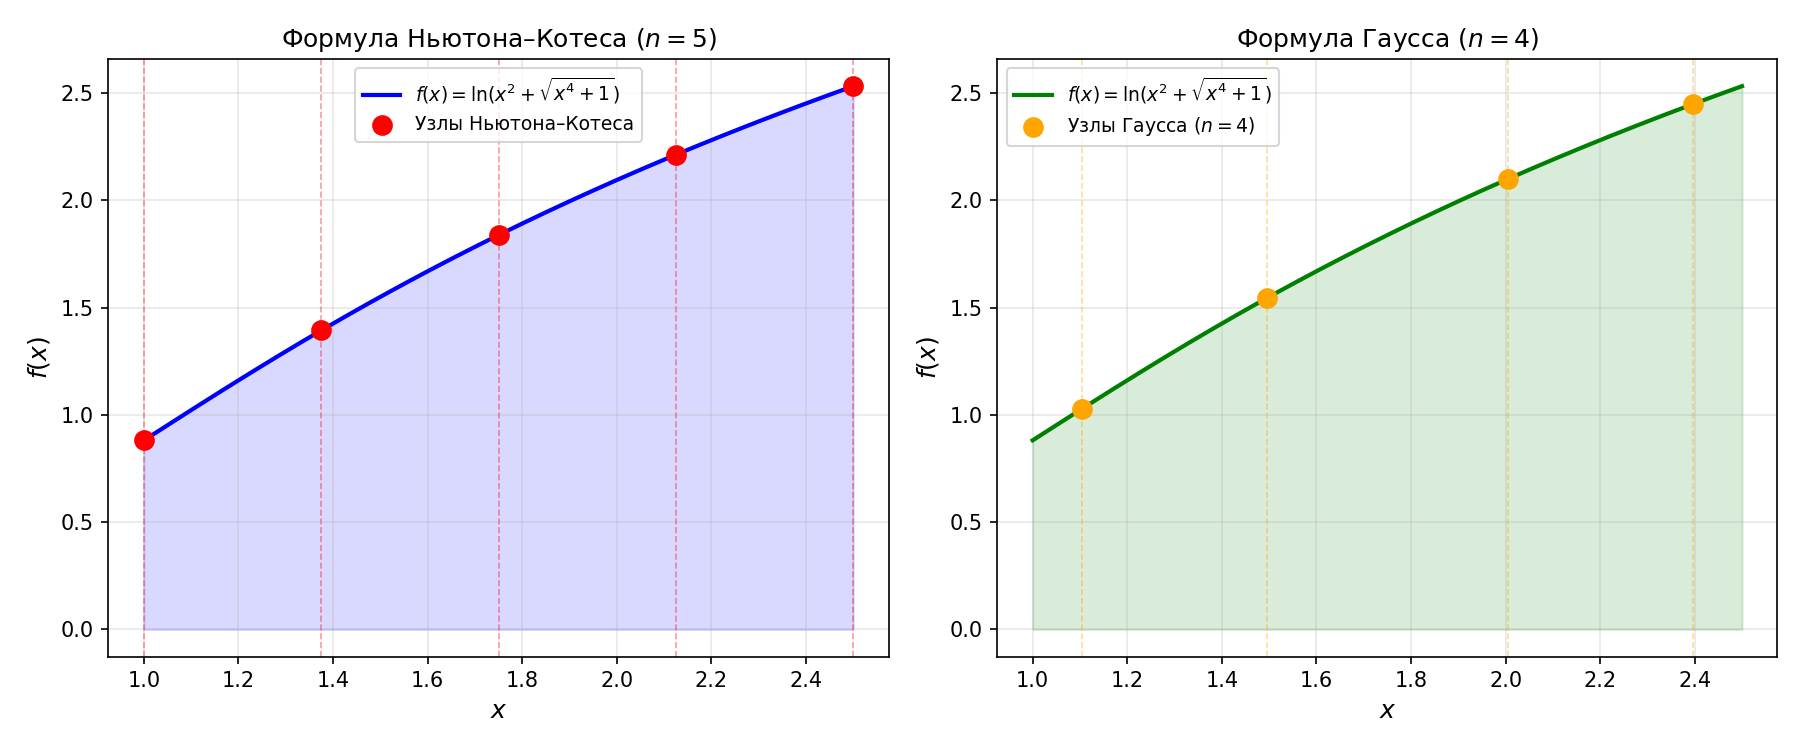
\includegraphics[width=\textwidth]{integration.png}
\caption{Подынтегральная функция $f(x) = \ln(x^2+\sqrt{x^4+1})$
         и узлы квадратурных формул.}
\label{fig:integration}
\end{figure}

На листинге~\ref{lst:plot} приведён код построения графика.

\begin{lstlisting}[caption={Построение графика}, label=lst:plot]
import matplotlib.pyplot as plt

x_plot  = np.linspace(a, b, 400)
y_plot  = f(x_plot)
nodes_nc = [1.0, 1.375, 1.75, 2.125, 2.5]
x_gauss  = [1.104148, 1.495014, 2.004986, 2.395852]

fig, axes = plt.subplots(1, 2, figsize=(12, 5))

# Ньютона-Котеса
ax = axes[0]
ax.fill_between(x_plot, 0, y_plot, alpha=0.15, color='blue')
ax.plot(x_plot, y_plot, 'b-', linewidth=2,
        label=r'$f(x)=\ln(x^2+\sqrt{x^4+1})$')
ax.scatter(nodes_nc, [f(xi) for xi in nodes_nc],
           color='red', s=80, zorder=5, label=r'Узлы $x_i$')
ax.set_title('Формула Ньютона-Котеса ($n=5$)')
ax.set_xlabel('$x$'); ax.set_ylabel('$f(x)$')
ax.legend(); ax.grid(True, alpha=0.3)

# Гаусса
ax = axes[1]
ax.fill_between(x_plot, 0, y_plot, alpha=0.15, color='green')
ax.plot(x_plot, y_plot, 'g-', linewidth=2,
        label=r'$f(x)=\ln(x^2+\sqrt{x^4+1})$')
ax.scatter(x_gauss, [f(xi) for xi in x_gauss],
           color='orange', s=80, zorder=5, label=r'Узлы $x_i$')
ax.set_title('Формула Гаусса ($n=4$)')
ax.set_xlabel('$x$'); ax.set_ylabel('$f(x)$')
ax.legend(); ax.grid(True, alpha=0.3)

plt.tight_layout()
plt.savefig('integration.png', dpi=150)
plt.show()
\end{lstlisting}

\newpage

% ============================================================
% conclusion
% ============================================================
\section*{Заключение}
\addcontentsline{toc}{section}{Заключение}

В ходе выполнения лабораторной работы было приближённо вычислено значение интеграла
\[
I = \int_{1}^{2{,}5} \ln\!\left(x^2 + \sqrt{x^4+1}\right)dx
\]
двумя квадратурными методами.

\textbf{Формула Ньютона-Котеса ($n=5$, формула Буля).}
Шаг $h = 0{,}375$. По формуле из таблицы~\ref{tab:nk}:
\[
I^*_\text{НК} = \frac{b-a}{90}\bigl[14f_0 + 64f_1 + 24f_2 + 64f_3 + 14f_4\bigr]
= 2{,}689230.
\]
Оценка предельной погрешности через остаточный член:
$\bigl|R^{(5)}\bigr| \leq 0{,}4548$.
Фактическая погрешность: $\Delta I^*_\text{НК} \approx 1{,}67\cdot10^{-4}$.

\textbf{Формула Гаусса ($n=4$).}
Узлы $t_i$ из таблицы~\ref{tab:gauss} пересчитаны на $[1;\,2{,}5]$
по формуле~\eqref{eq:gauss_nodes}. По формуле~\eqref{eq:gauss_formula}:
\[
I^*_\text{Г} = \frac{b-a}{2}\sum_{i=1}^{4} A_i\,f(x_i) = 0{,}75 \cdot 3{,}585417 = 2{,}689062.
\]
Погрешность относительно точного значения $I_\text{точн} \approx 2{,}689063$:
$\Delta I^*_\text{Г} \approx 6{,}0\cdot10^{-7}$.

Формула Гаусса при $n=4$ значительно точнее формулы Ньютона-Котеса при $n=5$
благодаря алгебраической степени точности $2n-1 = 7$.
Все вычисления выполнены программно на языке Python
с использованием библиотек NumPy и SciPy.

\end{document}